\section{The Chromatic Number Problem}\label{sec:chromatic}

\subsection{Estimating the Chromatic Number of a Graph}

Since the chromatic number problem is NP-hard, an alternative to finding an exact answer is to find lower and upper
bounds for the actual value.  If these bounds happen to match then they provide the actual chromatic number.  The
following sections describe well-known methods for finding the upper and lower bounds for the chromatic number of a
graph.

\subsubsection{Finding a Lower Bound}\label{sec:sub:sub:lower}

The most popular strategy for estimating a lower bound for the chromatic number of a graph is based on the
statement of \propname~\ref{prop:clique}.  For a graph \(G\):
\[\w^*(G)\le\w(G)\le\X(G)\]
where \(\w^*(G)\) is a lower bound estimate for the clique number of \(G\).  Another less popular bound is given by
\theoremname~\ref{thm:lbalpha}.

\begin{theorem}
  \label{thm:lbalpha}
  Let \(G\) be a graph of order \(n\).  \(\displaystyle \X(G)\ge\frac{n}{\a(G)}\).
\end{theorem}

\begin{proof}
  Assume that \(G\) is \chromatic{k}.  This means that \(V(G)\) can be partitioned into \(k\) non-empty independent
  sets \(A_1,\ldots,A_k\), where each \(\abs{A_i}\le\a(G)\).
  \[n=\abs*{\bigcup_{1\le i\le k}A_i}=\sum_{i=1}^k\abs{A_i}\le\sum_{i=1}^k\a(G)=k\a(G)\]
  Therefore, \(\displaystyle k\ge\frac{n}{\a(G)}\).
\end{proof}

Note that both of the above lower bounds are tight when \(G\) is complete.

It is well-known that certain triangle-free graphs with \(\w(G)=2\) can have arbitrarily high \(\X(G)\).  Examples
are the graphs created using the so-called \emph{Mycielski} construction~\cite{west}:
\begin{enumerate}
\item Start with \(G=P_2\) \((\X(G)=2)\).
\item\label{step:myc:repeat} For the vertices in \(v\in V(G)\), create new vertices \(U=\set{u_1,\ldots,u_n}\) such
  that \(N(u_i)=N(v_i)\).  The new vertices form what is referred to as a \emph{shadow} graph.
\item Add an additional vertex \(w\) such that \(N(w)=U\) and call this new graph \(G'\), which has
  \(\X(G')=\X(G)+1\).
\item Let \(G=G'\) and go to step~\ref{step:myc:repeat}.
\end{enumerate}

The first three graphs resulting from the Mycielski construction are shown in \figurename~\ref{fig:mycielski}.

\begin{figure}[H]
  \begin{minipage}{1in}
    \centering
    \scalebox{0.75}{
      \begin{tikzpicture}[every node/.style={labeled node}, node distance=1in]
        \pathV{\(v_1\),\(v_2\)}{(0,0)}{below};
      \end{tikzpicture}
    }

    \(k=2\)
  \end{minipage}
  \begin{minipage}{2in}
    \centering
    \scalebox{0.75}{
      \begin{tikzpicture}[every node/.style={labeled node}, node distance=1in]
        \cycleV{\(v_1\),\(v_2\),\(u_1\),\(w\),\(u_2\)}{(0,0)}{0.75in}{90}{};
      \end{tikzpicture}
    }

    \(k=3\)
  \end{minipage}
  \begin{minipage}{2.75in}
    \centering
    \scalebox{0.75}{
      \begin{tikzpicture}[every node/.style={labeled node}, node distance=1in]
        \cycleV{\(v_1\),\(v_2\),\(v_3\),\(v_4\),\(v_5\)}{(0,0)}{1.25in}{90}{o};
        \cycleV{\(u_1\),\(u_2\),\(u_3\),\(u_4\),\(u_5\)}{(0,0)}{0.75in}{90}{i};
        \draw (i1) edge (o5) edge (o2);
        \draw (i2) edge (o1) edge (o3);
        \draw (i3) edge (o2) edge (o4);
        \draw (i4) edge (o3) edge (o5);
        \draw (i5) edge (o4) edge (o1);
        \node (w) at (0,0) {\(w\)};
        \draw (w) edge (i1) edge (i2) edge (i3) edge (i4) edge (i5);
      \end{tikzpicture}
    }

    \(k=4\)
  \end{minipage}
  \caption{The first three graphs from the Mycielski construction.}
  \label{fig:mycielski}
\end{figure}

The third graph in \figurename~\ref{fig:mycielski} is called the \emph{Gr\"otzsch} graph.  For another example of
triangle free graphs with arbitrarily high chromatic number, see Zhang~\cite{zhang}.  Nevertheless, for the general
case the clique number is a suitable lower bound for the chromatic number.

Unfortunately, the clique number problem for a graph \(G\) is also NP-hard, so the next best step is to use a
P-time calculation for a \(\w^*(G)\) that is as tight as possible to the actual \(\w(G)\).  Edwards and
Elphick~(1982)~\cite{edwards} investigated several such methods and concluded that the best method was a simple
calculation based on the adjacency matrix of \(G\):
\begin{enumerate}
\item Select (either lowest index or at random) a vertex \(v\in V(G)\) of maximum degree in \(G\)
  \((\deg(v)=\dmax(G))\) and let \(S=\set{v}\).
\item\label{step:edw:select} Select the vertex \(v_i\in V(G)\) such that \(v_i\notin S\) and with the minimum index
  value \(i\) that is adjacent to all of the vertices in \(S\).  If no such vertex exists then go to
  step~\ref{step:edw:done}.
\item Add \(v_i\) to \(S\) and go to step~\ref{step:edw:select}.
\item\label{step:edw:done} \(G[S]\) is a complete subgraph of \(G\) so conclude that \(\w^*(G)=\abs{S}\le\w(G)\).
\end{enumerate}

The Edwards algorithm has \(\BO(n^2)\) runtime complexity and so it is a suitable P-time algorithm.

The results of a random graph analysis of the Edwards Elphick algorithm are shown in
\figurename~\ref{fig:edwards1err}.  The graph shows edge probability versus the mean of \(\w(G)-\w^*(G)\) for
graphs of increasing order with \(1000\) trials per edge probability.  Note that the error increases with both
order and edge probability.

\begin{figure}[H]
  \centering
  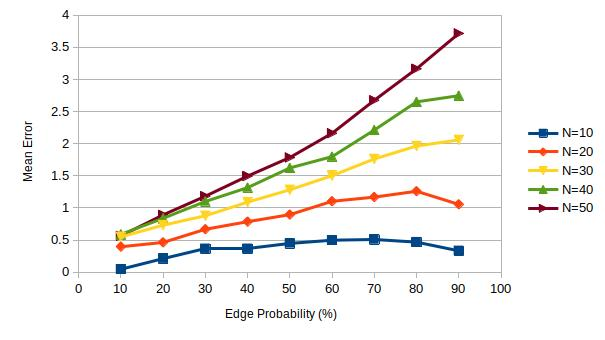
\includegraphics[width=5in]{edwards1_error}
  \caption{Edwards Elphick algorithm mean error.}
  \label{fig:edwards1err}
\end{figure}

Step~\ref{step:edw:select} of the algorithm selects the next vertex of lowest index that is adjacent to all
previously selected vertices.  An improvement would be to select a vertex with the highest degree that is adjacent
to all previously selected vertices.  This would of course increase the average runtime complexity to the worst
case of the unimproved algorithm, but it would still be P-time.  The results of this improved algorithm are shown
in \figurename~\ref{fig:edwards2err}.

\begin{figure}[H]
  \centering
  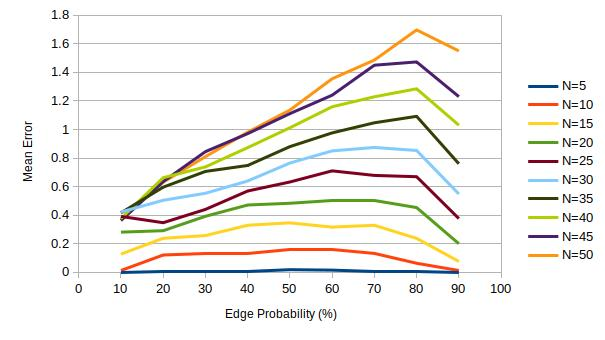
\includegraphics[width=5in]{edwards2_error}
  \caption{Improved Edwards Elphick algorithm mean error.}
  \label{fig:edwards2err}
\end{figure}

Note that the improved algorithm cuts the error in half.  The worst case time durations are shown in
\figurename~\ref{fig:edwards2time}. Clearly, execution time is very small.

\begin{figure}[H]
  \centering
  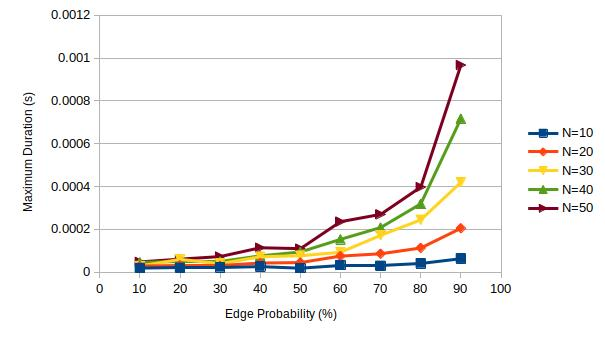
\includegraphics[width=5in]{edwards2_time}
  \caption{Improved Edwards Elphick algorithm maximum duration.}
  \label{fig:edwards2time}
\end{figure}

As will be shown later in this section, being able to compute the clique number of a graph, or at least a suitable
estimate, is an important bounding condition for many of the well-known algorithms for finding the chromatic number
of a graph.  Many of these algorithms rely on the statement of \theoremname~\ref{thm:isclique} that a maximal
clique in a graph \(G\) is a maximal independent set in \(\bar{G}\).  A nice summary of these algorithms is given
by Xiao and Nagamouchi~(2017)~\cite{xiao}.  They claim that the known algorithms tend to converge on a runtime
complexity of \(\BO(1.2^n)\).  These algorithms tend be somewhat complex and geared towards larger \(n\).

A simpler yet efficient alternative to these exact algorithms is the Bron Kerbosch algorithm~(1973)~\cite{bron}.
The advantage of the Bron Kerbosch (BK) algorithm is that it finds all possible maximal independent sets in a
graph, and hence can be used to find \(\a(G)=\w(\bar{G})\).  Finding all of the maximal independent sets in a graph
is a crucial part of the Christofides algorithm, which is discussed later in this section.

The heart of BK is a recursive subroutine called \emph{extend}, where the calls to \emph{extend} implement a
depth-first walk of an exhaustive search tree.  At each node in the search tree, three vertex lists are maintained:

\begin{description}
\item[compsub] The current maximal clique accumulator.
\item[candidates] A set of vertices that can be added to \emph{compsub}.
\item[old] A set of vertices that already have been used in the current search branch.
\end{description}

The initial call is seeded with an empty \emph{compsub} and all of the graph's vertices in \emph{candidates}.  Each
call to \emph{extend} selects a vertex from \emph{candidate}, adds it to \emph{compsub}, constructs new
\emph{candidates} and \emph{old} sets by removing vertices that are not adjacent to the selected vertex, and then
calls itself with the new lists.  The termination leaf for each branch is when \emph{candidates} is empty.  If
\emph{old} is also empty then \emph{compsub} contains a new maximal clique.  Otherwise, the clique in
\emph{compsub} is a subset of an earlier found clique that contains the vertices in \emph{old} and thus is not
maximal.  Upon each return from a call to \emph{extend}, the corresponding candidate is removed from \emph{compsub}
and is added to \emph{old}.

A small improvement added to BK by this research is to abandon the current branch when the desire is to only find
\(\a(G)\) and the number of vertices in \emph{compsub} and \emph{candidates} are not enough to build a maximal
clique larger than all previously found maximal cliques.

Bron and Kerbosch actually propose two variations of the algorithm that differ by how the next vertex is selected
from \emph{candidates}.  In the basic mode, any such vertex may be selected.

\subsubsection{Finding an Upper Bound}\label{sec:sub:sub:upper}

\subsection{The Christofides Algorithm}\label{sec:sub:christofides}

\subsection{Zykov Algorithms}\label{sec:sub:zykov}

An exhaustive, exponential-time algorithm for determining the chromatic number of a graph is derived from a
nondeterministic Turing machine technique attributed to Ukranian graph theorist Alexandre A. Zykov (1922--2013)
\cite{obit}.

\begin{figure}[h]
  \label{fig:zykov}
  \begin{center}
    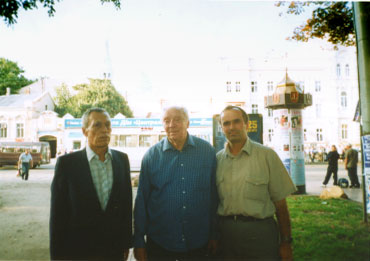
\includegraphics{zykov}
  \end{center}
  \caption{V.G Vizing (L), A.A. Zykov (C), and V.I. Voloshin (R) in Odessa (2001) \cite{voloshin}}
\end{figure}

\subsubsection{The Chromatic Polynomial}

In his 1949 paper (translated by the AMS in 1952) \cite{zykov}, Zykov addresses the question: given a graph \(G\) and
a number \(k\in\N\), how many ways are there to properly color \(G\) using at most \(k\) colors?  In fact, he is not
particularly concerned about the chromatic number, which he calls the \emph{rank}, of a graph.  To solve this problem,
Zykov notes that in any proper coloring of a graph:
\begin{enumerate}
\item Nonadjacent vertices have either the same color or different colors.
\item Adjacent vertices always have different colors.
\end{enumerate}
If nonadjacent vertices have the same color then they can be contracted and the resulting graph retains the same
\coloring{k} as the original graph.  This is demonstrated in Figure \ref{fig:zvcon}.

\begin{figure}[h]
  \label{fig:zvcon}
  \begin{center}
    \begin{minipage}{2in}
      \begin{center}
        \begin{tikzpicture}[every node/.style={labeled node}]
          \colorlet{c1}{green!25!white}
          \colorlet{c2}{blue!25!white}
          \colorlet{c3}{red!25!white}
          \node (d) [fill=c2] at (0,0) {\(d\)};
          \node (c) [fill=c3,right=of d] {\(c\)};
          \node (b) [fill=c2,above=of c] {\(b\)};
          \node (a) [fill=c1,above=of d] {\(a\)};
          \draw (a) -- (b);
          \draw (a) -- (c) -- (d) -- (a);
        \end{tikzpicture}

        \bigskip

        \(G\)
      \end{center}
    \end{minipage}
    \begin{minipage}{2in}
      \begin{center}
        \begin{tikzpicture}[every node/.style={labeled node}]
          \colorlet{c1}{green!25!white}
          \colorlet{c2}{blue!25!white}
          \colorlet{c3}{red!25!white}
          \node (bd) [fill=c2] at (0,0) {\(bd\)};
          \node (c) [fill=c3,right=of bd] {\(c\)};
          \node (a) [fill=c1,above=of bd] {\(a\)};
          \draw (a) -- (c) -- (bd) -- (a);
        \end{tikzpicture}

        \bigskip

        \(G\cdot bd\)
      \end{center}
    \end{minipage}
  \end{center}
  \caption{Same Colors with Vertex Contraction}
\end{figure}

If nonadjacent vertices have different colors then they can be joined by an edge and the resulting graph retains
the same \coloring{k} as the original graph.  This is demonstrated in Figure \ref{fig:zeadd}.

\begin{figure}[h]
  \label{fig:zeadd}
  \begin{center}
    \begin{minipage}{2in}
      \begin{center}
        \begin{tikzpicture}[every node/.style={labeled node}]
          \colorlet{c1}{green!25!white}
          \colorlet{c2}{blue!25!white}
          \colorlet{c3}{red!25!white}
          \node (d) [fill=c2] at (0,0) {\(d\)};
          \node (c) [fill=c3,right=of d] {\(c\)};
          \node (b) [fill=c2,above=of c] {\(b\)};
          \node (a) [fill=c1,above=of d] {\(a\)};
          \draw (a) -- (b);
          \draw (a) -- (c) -- (d) -- (a);
        \end{tikzpicture}

        \bigskip

        \(G\)
      \end{center}
    \end{minipage}
    \begin{minipage}{2in}
      \begin{center}
        \begin{tikzpicture}[every node/.style={labeled node}]
          \colorlet{c1}{green!25!white}
          \colorlet{c2}{blue!25!white}
          \colorlet{c3}{red!25!white}
          \node (d) [fill=c2] at (0,0) {\(d\)};
          \node (c) [fill=c3,right=of d] {\(c\)};
          \node (b) [fill=c2,above=of c] {\(b\)};
          \node (a) [fill=c1,above=of d] {\(a\)};
          \draw (a) -- (b) -- (c);
          \draw (a) -- (c) -- (d) -- (a);
        \end{tikzpicture}

        \bigskip

        \(G+bc\)
      \end{center}
    \end{minipage}
  \end{center}
  \caption{Different Colors with Edge Addition}
\end{figure}

By applying these steps recursively, all of the possible distributions of the nonadjacent nodes to independent sets
are generated.  The termination condition for each recursive path is a complete graph of some varying order \(k\).
Each node in the complete graph represents an independent set of nonadjacent nodes in the original graph that have
been combined via vertex contraction.  Thus, each complete graph of order \(k\) represents a possible \coloring{k}
of the original graph.  The complete graphs of smallest order represent chromatic colorings and their order is the
chromatic number of the original graph.

Zykov uses a graph equation syntax to record the recursive processing of a graph, where each line in the equation
represents the next recursive layer.  Isomorphic graphs are combined with a frequency multiplier at each layer.
This is demonstrated in Figure \ref{fig:greqn}.

\begin{figure}[h]
  \label{fig:greqn}
  \begin{align*}
    \begin{minipage}{0.75in}
      \begin{center}
        \begin{tikzpicture}[every node/.style={unlabeled node}]
          \node (a1) at (0,0) {};
          \node (a2) [right=of a1] {};
          \node (a3) [above=of a2] {};
          \node (a4) [above=of a1] {};
          \draw (a3) -- (a4) -- (a1) -- (a2) -- (a4);
        \end{tikzpicture}
      \end{center}
    \end{minipage} &=
    \begin{minipage}{0.75in}
      \begin{center} 
        \begin{tikzpicture}[every node/.style={unlabeled node}]
          \node (b1) at (0,0) {};
          \node (b2) [above=of b1] {};
          \node (b3) [right=of b1] {};
          \draw (b1) -- (b2) -- (b3) -- (b1);
        \end{tikzpicture}
      \end{center}
    \end{minipage} +
    \begin{minipage}{0.75in}
      \begin{center}
        \begin{tikzpicture}[every node/.style={unlabeled node}]
          \node (c1) at (0,0) {};
          \node (c2) [right=of a1] {};
          \node (c3) [above=of a2] {};
          \node (c4) [above=of a1] {};
          \draw (c2) -- (c3) -- (c4) -- (c1) -- (c2) -- (c4);
        \end{tikzpicture}
      \end{center}
    \end{minipage} \\
    &= \begin{minipage}{0.75in}
      \begin{center} 
        \begin{tikzpicture}[every node/.style={unlabeled node}]
          \node (b1) at (0,0) {};
          \node (b2) [above=of b1] {};
          \node (b3) [right=of b1] {};
          \draw (b1) -- (b2) -- (b3) -- (b1);
        \end{tikzpicture}
      \end{center}
    \end{minipage} +
    \begin{minipage}{0.75in}
      \begin{center} 
        \begin{tikzpicture}[every node/.style={unlabeled node}]
          \node (b1) at (0,0) {};
          \node (b2) [above=of b1] {};
          \node (b3) [right=of b1] {};
          \draw (b1) -- (b2) -- (b3) -- (b1);
        \end{tikzpicture}
      \end{center}
    \end{minipage} +
    \begin{minipage}{0.75in}
      \begin{center}
        \begin{tikzpicture}[every node/.style={unlabeled node}]
          \node (c1) at (0,0) {};
          \node (c2) [right=of a1] {};
          \node (c3) [above=of a2] {};
          \node (c4) [above=of a1] {};
          \draw (c2) -- (c3) -- (c4) -- (c1) -- (c2) -- (c4);
          \draw (c1) -- (c3);
        \end{tikzpicture}
      \end{center}
    \end{minipage} \\
    &= 2
    \begin{minipage}{0.75in}
      \begin{center} 
        \begin{tikzpicture}[every node/.style={unlabeled node}]
          \node (b1) at (0,0) {};
          \node (b2) [above=of b1] {};
          \node (b3) [right=of b1] {};
          \draw (b1) -- (b2) -- (b3) -- (b1);
        \end{tikzpicture}
      \end{center}
    \end{minipage} +
    \begin{minipage}{0.75in}
      \begin{center}
        \begin{tikzpicture}[every node/.style={unlabeled node}]
          \node (c1) at (0,0) {};
          \node (c2) [right=of a1] {};
          \node (c3) [above=of a2] {};
          \node (c4) [above=of a1] {};
          \draw (c2) -- (c3) -- (c4) -- (c1) -- (c2) -- (c4);
          \draw (c1) -- (c3);
        \end{tikzpicture}
      \end{center}
    \end{minipage} \\
    &= 2K_3+K_4
  \end{align*}
  \caption{Zykov Graph Equation}
\end{figure}

Determining whether two graphs are isomorphic is hard, so combining isomorphic graphs in all but the very simple
cases should be skipped; the complete graphs resulting from the further processing of two isomorphic graphs will
eventually be combined anyway by the end.

Zykov was trying to determine the number of \coloring{k}s of a graph without color indifference: each permutation
of colors for a particular distribution is considered unique.  Thus, Zykov multiplied each complete graph
coefficient in the final line of a graph equation by the number of permutations from selecting the order \(n\) of
the particular complete graph from \(k\) colors:
\[k^{(n)}=k(k-1)(k-2)\cdots(k-n+1)\]
Thus, the total number of unique colorings from the example shown in Figure \ref{fig:greqn} using \(k\) colors
would be:
\[M(G,k)=2k^{(3)}+k^{(4)}\]
This is known as the factorial form of the \emph{chromatic polynomial} for the graph.  The corresponding
\emph{expanded form} is:
\[M(G,k)=k^4-4k^3+5k^2-2k\]
Read (1968) \cite{read} expands on the construction of the factorial form of the chromatic polynomial for a graph
and proves several theorems regarding the expanded form.  Some examples are:
\begin{enumerate}
\item \(M(G,k)=M(G\cdot uv)+M(G+uv)\), where \(u\) and \(v\) are any two nonadjacent vertices in the current
  recursive step.
\item The degree of M(G,k) is the order of \(G\).
\item The highest order coefficient is \(1\).
\item There is no constant term.
\item The terms alternate in sign.
\end{enumerate}
In fact, Read shows that the expanded form is actually an inclusion-exclusion equation resulting from starting with
all possible proper and improper colorings \(k^n\) and then subtracting the improper colorings.

\subsubsection{An Exhaustive Algorithm}

Corneil and Graham extend Zykov's work with the following theorem \cite{corneil}:

\begin{theorem}[Corneil and Graham, 1973]
  \label{thm:corneil}
  Let \(G\) be a graph and let \(u\) and \(v\) be two nonadjacent vertices in \(G\):
  \[\X(G)=\min\set{\X(G\cdot uv),\X(G+uv)}\]
\end{theorem}

Zykov's method combined with Theorem \ref{thm:corneil} can be used to construct an exhaustive algorithm for finding
the chromatic number and a chromatic coloring for a graph \(G\).  We define \(S\) to be a first-in-first out (FIFO)
stack of graphs and \(X\) to be the last found complete graph of the smallest order.  Each vertex in \(X\)
represents a set of contracted vertices.
\begin{enumerate}
\item Construct a graph \(G'\) that is isomorphic to \(G\) and where each vertex in \(G'\) is a list of contracted
  vertices initialized to a one element list containing the corresponding vertex in \(G\).
\item Push \(G'\) onto \(S\).
\item \label{step:zempty} If \(S\) is empty then return \(n(X)\) and \(X\).
\item \label{step:zcheck} If the graph on the top of \(S\) is complete:
  \begin{enumerate}
  \item Pop the graph off of the top of \(S\) and save it as \(H\).
  \item If \(X\) is not set or \(n(H)<n(X)\) then let \(X=H\).  Otherwise, discard \(H\).
  \item Go to step \ref{step:zempty}.
  \end{enumerate}
\item The graph on the top of \(S\) is not complete.  Pop the graph off of \(S\) and save it as \(H\).
\item Pick any two nonadjacent vertices \(u\) and \(v\) in \(H\).
\item Push \(H+uv\) onto \(S\).
\item Construct \(H'=H\cdot uv\), where the contracted vertex list for the new contracted vertex is a concatenation
  of the lists for \(u\) and \(v\).
\item Push \(H'\) onto \(S\).
\item Go to step \ref{step:zcheck}.
\end{enumerate}

The steps of this algorithm can be tracked via a so-called \emph{Zykov tree} \cite{corneil}.  The Zykov tree for
the example in Figure \ref{fig:greqn} is shown in Figure \ref{fig:ztree}.  Note that the exhaustive algorithm
corresponds to a depth-first walk of the tree.

\begin{figure}[h]
  \label{fig:ztree}
  \begin{center}
    \begin{tikzpicture}
      \node (a) [draw,circle] at (0,0) {
        \begin{tikzpicture}[every node/.style={unlabeled node}]
          \node (a1) at (0,0) {};
          \node (a2) [right=of a1] {};
          \node (a3) [above=of a2] {};
          \node (a4) [above=of a1] {};
          \draw (a3) -- (a4) -- (a1) -- (a2) -- (a4);
        \end{tikzpicture}
      };
      \node (b) [draw,circle,below left=of a] {
        \begin{tikzpicture}[every node/.style={unlabeled node}]
          \node (b1) at (0,0) {};
          \node (b2) [above=of b1] {};
          \node (b3) [right=of b1] {};
          \draw (b1) -- (b2) -- (b3) -- (b1);
        \end{tikzpicture}
      };
      \node (c) [draw,circle,below right=of a] {
        \begin{tikzpicture}[every node/.style={unlabeled node}]
          \node (c1) at (0,0) {};
          \node (c2) [right=of a1] {};
          \node (c3) [above=of a2] {};
          \node (c4) [above=of a1] {};
          \draw (c2) -- (c3) -- (c4) -- (c1) -- (c2) -- (c4);
        \end{tikzpicture}
      };
      \node (d) [draw,circle,below left=of c] {
        \begin{tikzpicture}[every node/.style={unlabeled node}]
          \node (d1) at (0,0) {};
          \node (d2) [above=of d1] {};
          \node (d3) [right=of d1] {};
          \draw (d1) -- (d2) -- (d3) -- (d1);
        \end{tikzpicture}
      };
      \node (e) [draw,circle,below right=of c] {
        \begin{tikzpicture}[every node/.style={unlabeled node}]
          \node (c1) at (0,0) {};
          \node (c2) [right=of a1] {};
          \node (c3) [above=of a2] {};
          \node (c4) [above=of a1] {};
          \draw (c2) -- (c3) -- (c4) -- (c1) -- (c2) -- (c4);
          \draw (c1) -- (c3);
        \end{tikzpicture}
      };
      \draw (a) edge (b) edge (c);
      \draw (c) edge (d) edge (e);
    \end{tikzpicture}
  \end{center}
  \caption{A Zykov Tree}
\end{figure}

\subsubsection{Branch and Bound Strategies}

Using a Zykov tree suggests that the exhaustive algorithm is a candidate for a branch-and-bound solution, where the
branching is accomplished via vertex contraction and edge addition and the bounding is some method to prematurely
terminate a branch.  Corneil and Graham suggest such a bounding technique through the determination of so-called
\(\a\)-clusters; however, the algorithm for finding such clusters has \(\BO(n^3)\) runtime complexity.
